\documentclass[11pt,a4paper]{article}
\usepackage[T1]{fontenc}
\usepackage[utf8]{inputenc}
\usepackage{lmodern}
\usepackage[margin=2.3cm]{geometry}
\usepackage{graphicx}
\graphicspath{{../img/}}
\usepackage{xcolor}
\definecolor{spblue}{HTML}{1F4E79}
\definecolor{spteal}{HTML}{2C7A7B}
\usepackage{booktabs}
\usepackage{longtable}
\usepackage{array}
\usepackage{enumitem}
\usepackage{float}
\usepackage{caption}
\captionsetup{font=small,labelfont=bf}
\usepackage{listings}
\lstset{basicstyle=\ttfamily\footnotesize,breaklines=true,frame=single,backgroundcolor=\color{gray!8},columns=fullflexible,keepspaces=true}
\usepackage[hidelinks]{hyperref}
\usepackage{titlesec}
\titleformat{\section}{\color{spblue}\Large\bfseries}{\thesection}{0.6em}{}
\titleformat{\subsection}{\color{spteal}\large\bfseries}{\thesubsection}{0.6em}{}
\setlength{\parskip}{0.5em}\setlength{\parindent}{0pt}

\title{ScholarPath --- From ERD to EERD\\[0.3em]\large Step 2: Enhancement}
\author{ScholarPath Team}
\date{}

\begin{document}
\maketitle

\begin{abstract}
This is Part~2 of a four-part teaching series that walks the ScholarPath data
model through the classical database-design pipeline: plain ERD $\rightarrow$
Enhanced Entity--Relationship diagram (EERD) $\rightarrow$ relational mapping
$\rightarrow$ class diagrams. Building on the conceptual ERD established in
Part~1, this document enriches that model into a full \emph{Enhanced} ER diagram
using the constructs of the Extended ER model (Elmasri \& Navathe):
specialization / generalization, disjointness and completeness constraints, weak
entities, multivalued and derived attributes, and categories. We apply each
construct to the actual ScholarPath schema --- grounded in the live EF~Core model
snapshot and the domain entities --- and we state one project-specific notation
convention (solid versus dashed edges) so the diagrams cannot be misread by the
defense committee. We close by previewing Part~3, the relational mapping.
\end{abstract}

\tableofcontents

\bigskip

\section{Recap of Part 1 and the Goal of This Step}

Part~1 (\emph{ScholarPath --- The Entity--Relationship Diagram}) established the
plain conceptual ERD: it identified the core entity types of the platform ---
\texttt{USERS}, \texttt{SCHOLARSHIP}, \texttt{APPLICATION}, \texttt{BOOKING},
\texttt{PAYMENT}, \texttt{FORUM\_POST}, \texttt{RESOURCE},
\texttt{NOTIFICATION}, \texttt{AI\_INTERACTION} and their neighbours --- together
with the relationship types that connect them and the cardinality ratios
(1:1, 1:N, M:N) on each. That diagram answered the question \emph{``what things
exist and how are they related?''} at the level any introductory ER textbook
would recognise: rectangles for entities, diamonds for relationships, ovals for
attributes.

A plain ERD, however, cannot express several facts that are genuinely true of
ScholarPath. It has no symbol for the idea that a single principal can
simultaneously be a Student \emph{and} a Consultant; it cannot say that an
education entry has no independent existence without its owning profile; and it
cannot distinguish an attribute that is physically stored from one that is
\emph{computed} on the fly. These are exactly the gaps the Enhanced ER model
was designed to fill.

\textbf{Goal of Step~2.} Take the Part~1 ERD and \emph{enrich} it into an EERD by
adding the four ``enhancement'' constructs --- specialization/generalization,
weak entities, multivalued attributes, and derived attributes --- plus one
project-specific edge-style convention. Every enhancement in this document is
grounded in the real model: the source of truth is the live EF~Core model
snapshot\\
\texttt{server/src/ScholarPath.Infrastructure/Migrations/ApplicationDbContextModelSnapshot.cs}\\
together with the domain entities under
\texttt{server/src/ScholarPath.Domain/Entities/}. We do not invent entities or
columns. The conceptual EERD is drawn in authentic Chen / Elmasri notation; the
companion documents \texttt{02-RELATIONAL-MAPPING.md} (Part~3) and the
class-diagram document (Part~4) continue from here.

\section{The EER Toolbox (Elmasri \& Navathe)}

The Extended (or Enhanced) ER model adds a small, well-defined vocabulary on top
of the basic ERD. We summarise the constructs we will use, then apply them in
Section~\ref{sec:apply}.

\subsection{Specialization and Generalization (ISA)}

A \textbf{superclass} (super-type) is an entity type whose members can be divided
into \textbf{subclasses} (sub-types) that share the superclass's attributes but
add their own. The relationship between a subclass and its superclass is the
\textbf{IS-A} relationship, drawn in Elmasri notation with a circle joined to the
superclass and a subset symbol ($\subset$) on each subclass line.

\begin{itemize}[leftmargin=1.4em]
  \item \textbf{Specialization} is the top-down act of defining subclasses of a
        superclass (e.g.\ a \texttt{USER} is specialized into Student / Company /
        Consultant / Admin).
  \item \textbf{Generalization} is the bottom-up act of recognising a common
        superclass for several entity types.
\end{itemize}

\subsection{Disjointness and Completeness Constraints}

Two orthogonal constraints qualify any specialization:

\begin{itemize}[leftmargin=1.4em]
  \item \textbf{Disjointness} --- written in the specialization circle:
        \begin{itemize}[leftmargin=1.4em]
          \item \textbf{disjoint \texttt{\{d\}}}: an entity instance belongs to
                \emph{at most one} subclass;
          \item \textbf{overlapping \texttt{\{o\}}}: an entity instance may
                belong to \emph{several} subclasses at once.
        \end{itemize}
  \item \textbf{Completeness} --- shown by the line from superclass to circle:
        \begin{itemize}[leftmargin=1.4em]
          \item \textbf{total} (double line): \emph{every} superclass instance
                must belong to at least one subclass;
          \item \textbf{partial} (single line): a superclass instance \emph{need
                not} belong to any subclass.
        \end{itemize}
\end{itemize}

\subsection{Weak Entities}

A \textbf{weak entity type} cannot be identified by its own attributes alone; its
existence and identification depend on an \emph{owner} (identifying) entity,
through an \emph{identifying relationship}. A weak entity has only a
\textbf{partial key} (discriminator) and is drawn with a double rectangle. In a
relational schema, weak entities become child tables whose primary key includes
(or whose existence is gated by) the owner's key, typically with a
\texttt{CASCADE} delete rule.

\subsection{Multivalued and Derived Attributes}

\begin{itemize}[leftmargin=1.4em]
  \item A \textbf{multivalued} attribute can hold a \emph{set} of values for one
        entity instance (double oval). Classic relational mapping breaks it out
        into a separate table; a pragmatic modern alternative is to store the set
        as a JSON-encoded column.
  \item A \textbf{derived} attribute (dashed oval) is \emph{computed} from other
        stored data rather than stored independently --- e.g.\ an average, a
        count, or a percentage.
\end{itemize}

\subsection{Categories (Union Types)}

A \textbf{category} (or union type) is a subclass whose members are drawn from the
union of \emph{several distinct} superclasses --- the EER answer to a
``polymorphic'' reference that can point at one of many entity types. ScholarPath
has two such polymorphic references (the knowledge-base source and the audit-log
target, Section~\ref{sec:cluster-ai}); rather than model them as a formal
category with a surrogate key, the platform realises them honestly as
\emph{loose} polymorphic id columns, which the next section makes explicit.

\section{Applying the EER Model to ScholarPath: the USER Super-type}
\label{sec:apply}

The single most important enhancement in ScholarPath is the specialization of the
central \texttt{USER} entity. Conceptually a \texttt{USER} is a superclass
specialized into four subclasses --- \textbf{Student}, \textbf{Company},
\textbf{Consultant}, and \textbf{Admin} --- each adding its own role-specific
attributes (Figure~\ref{fig:spec}).

\begin{figure}[H]\centering

\includegraphics[width=\linewidth,height=0.82\textheight,keepaspectratio]{eer-specialization.pdf}
\caption{The \texttt{USER} super-type specialized into Student, Company,
Consultant and Admin in authentic Elmasri \& Navathe EER notation. The
specialization circle carries \texttt{o} (overlapping); the single line from
\texttt{USER} to the circle marks partial participation; each subset symbol
($\subset$) reads ``\emph{subclass} IS-A USER''.}
\label{fig:spec}
\end{figure}

\subsection{The Two Constraints: Overlapping and Partial}

\textbf{Overlapping \texttt{\{o\}}.} The specialization is \emph{overlapping}, not
disjoint: a user may hold \emph{more than one} role at the same time. The
canonical case is a Student who is later upgraded to Consultant and keeps both
roles, so the same principal participates in the Student and Consultant
subclasses simultaneously. This rules out the disjoint \texttt{\{d\}} constraint.

\textbf{Partial.} The specialization is \emph{partial}, not total: a
freshly-registered user starts in the \texttt{Unassigned} state and belongs to
\emph{no} subclass until role selection / onboarding completes. Because at least
one valid \texttt{USER} instance (an unassigned newcomer) belongs to no subclass,
the participation of the superclass in the specialization is partial (single
line to the circle).

\subsection{How the Specialization Maps to the Physical Schema}

The EER picture above is the \emph{conceptual} view. Its physical realization in
the ScholarPath schema is deliberately a \textbf{single-table} mapping, not the
textbook table-per-subclass:

\begin{itemize}[leftmargin=1.4em]
  \item There is \textbf{no table-per-subclass}. The superclass is the single
        \texttt{Users} table.
  \item Role membership is the \textbf{\texttt{UserRoles}} join --- the ASP.NET
        Identity many-to-many between \texttt{Users} and \texttt{Roles}. The
        seeded roles are exactly \texttt{Admin}, \texttt{Student},
        \texttt{Company}, \texttt{Consultant}, \texttt{Unassigned}. Because the
        join allows several rows per user, it is precisely what makes the
        specialization \emph{overlapping}.
  \item The role-specific attributes --- Student academic fields, Company
        organization fields, Consultant expert fields --- are \emph{all columns
        on the single \texttt{UserProfiles} table}. For any given user, the
        columns belonging to the inapplicable sub-types are simply left
        \texttt{NULL}. This is the single-table (one relation for the whole
        hierarchy) realization of the specialization.
\end{itemize}

So the ``Enhanced'' modelling honestly captures the dual-role reality, while the
storage strategy keeps a single principal row --- consistent with the
\texttt{UserProfiles} columns seen in Section~\ref{sec:cluster-identity}
(\texttt{AcademicLevel}, \texttt{Gpa}, \texttt{OrganizationLegalName},
\texttt{SessionFeeUsd}, \texttt{StripeConnectStatus}).

\section{Other EER Constructs in ScholarPath}

Beyond specialization, three more enhancement constructs appear throughout the
model.

\subsection{Weak Entities}

Several child entity types have no independent existence and are owned by a parent
through an identifying relationship with a \texttt{CASCADE} delete rule:

\begin{itemize}[leftmargin=1.4em]
  \item \textbf{Education entries} (\texttt{EDUCATION\_ENTRIES}) depend on the
        owning \texttt{USER\_PROFILE} --- an education row is meaningless without
        its profile.
  \item \textbf{Scholarship child rows} (\texttt{SCHOLARSHIP\_CHILDREN}, cascade)
        and \textbf{application child rows} (\texttt{APPLICATION\_CHILDREN} ---
        status history, notes and tasks, cascade) exist only relative to their
        parent \texttt{SCHOLARSHIP} / \texttt{APPLICATION}.
  \item \textbf{Upgrade-request attachments}
        (\texttt{UPGRADE\_REQUEST\_FILES}, \texttt{UPGRADE\_REQUEST\_LINKS}) are
        attached to, and identified by, their parent \texttt{UPGRADE\_REQUEST}.
\end{itemize}

\subsection{Multivalued Attributes}

The Student subclass's \textbf{preferred countries} is a true multivalued
attribute --- a student may target several destination countries. Rather than
break it into a separate table, ScholarPath stores the set as a JSON-encoded
column on \texttt{UserProfiles} (mirroring \texttt{ExpertiseTagsJson} for
consultants). This is the pragmatic JSON realization of a multivalued attribute,
drawn in the conceptual diagram as the double-oval
\texttt{PreferredCountries}~\texttt{<<multi>>}.

\subsection{Derived Attributes}

Four attributes in the model are \emph{computed}, not independently authored, and
appear in the conceptual diagram as dashed ovals:

\begin{itemize}[leftmargin=1.4em]
  \item \texttt{CompanyAverageRating} --- the company's mean rating, derived from
        its \texttt{COMPANY\_REVIEWS}.
  \item \texttt{UpvoteCount} --- a forum post's net upvotes, cached on
        \texttt{FORUM\_POST} but derived from \texttt{FORUM\_VOTES}.
  \item \texttt{ProfileCompletenessPercent} --- a profile-fill percentage on
        \texttt{USER\_PROFILE}, derived from which fields are populated.
  \item \texttt{CostUsd} --- the per-call AI cost on \texttt{AI\_INTERACTION},
        derived from the prompt / completion token counts and the model's price.
\end{itemize}

\section{A Project-Specific Notation: Solid vs Dashed Edges}
\label{sec:notation}

ScholarPath adds one convention beyond the standard EER vocabulary, and it is
important enough to state explicitly so the diagrams cannot be misread.

\begin{longtable}{@{}p{3.2cm}p{11cm}@{}}
\toprule
\textbf{Line style} & \textbf{Meaning in this project} \\
\midrule
\endhead
\textbf{Solid} (\texttt{-{}-}) & A \textbf{database-enforced foreign key} --- a
real \texttt{FOREIGN KEY} constraint with a declared delete rule
(\texttt{Restrict}, \texttt{Cascade} or \texttt{SetNull}). \\
\textbf{Dashed} (\texttt{..}) & An \textbf{application-enforced ``loose''
reference} --- a \texttt{Guid} column that \emph{semantically} points at another
row but has \textbf{no FK constraint} in the schema. Referential integrity is
guaranteed by application code, not by the database. \\
\bottomrule
\end{longtable}

The platform deliberately uses loose references for high-volume, audit, log and
analytics tables --- notifications, votes, chat, audit log, AI interactions, and
payments / payouts --- so that deleting or anonymising a user never
cascade-breaks history. Modelling them honestly is part of an accurate EERD; for
example, \texttt{PAYMENT} and \texttt{PAYOUT} carry \emph{zero} DB-enforced
foreign keys, decoupling them from the principals for audit retention.

\textbf{Note for examiners.} In \emph{standard} crow's-foot notation a solid line
denotes an \emph{identifying} relationship and a dashed line a
\emph{non-identifying} one. Here we deliberately \textbf{repurpose} that visual
distinction to mean \textbf{DB-enforced FK (solid)} versus
\textbf{application-enforced loose reference (dashed)}. This is a project-specific
convention, stated up front so the diagrams cannot be misinterpreted.

\section{The Conceptual EERD and Its Subject-Area Clusters}

\subsection{The Full Conceptual EERD (Chen / Elmasri Notation)}

Figure~\ref{fig:core} is the consolidated conceptual EERD in authentic Chen /
Elmasri notation: rectangles are entity types, diamonds are relationship types,
ovals are attributes, underlined ovals are keys, double ovals are multivalued
attributes, dashed ovals are derived attributes, double lines mark total
participation and single lines partial participation, and \texttt{1 / N} are the
cardinality ratios. It is the master conceptual model from which the six
per-cluster detail diagrams below are drawn.

\begin{figure}[H]\centering
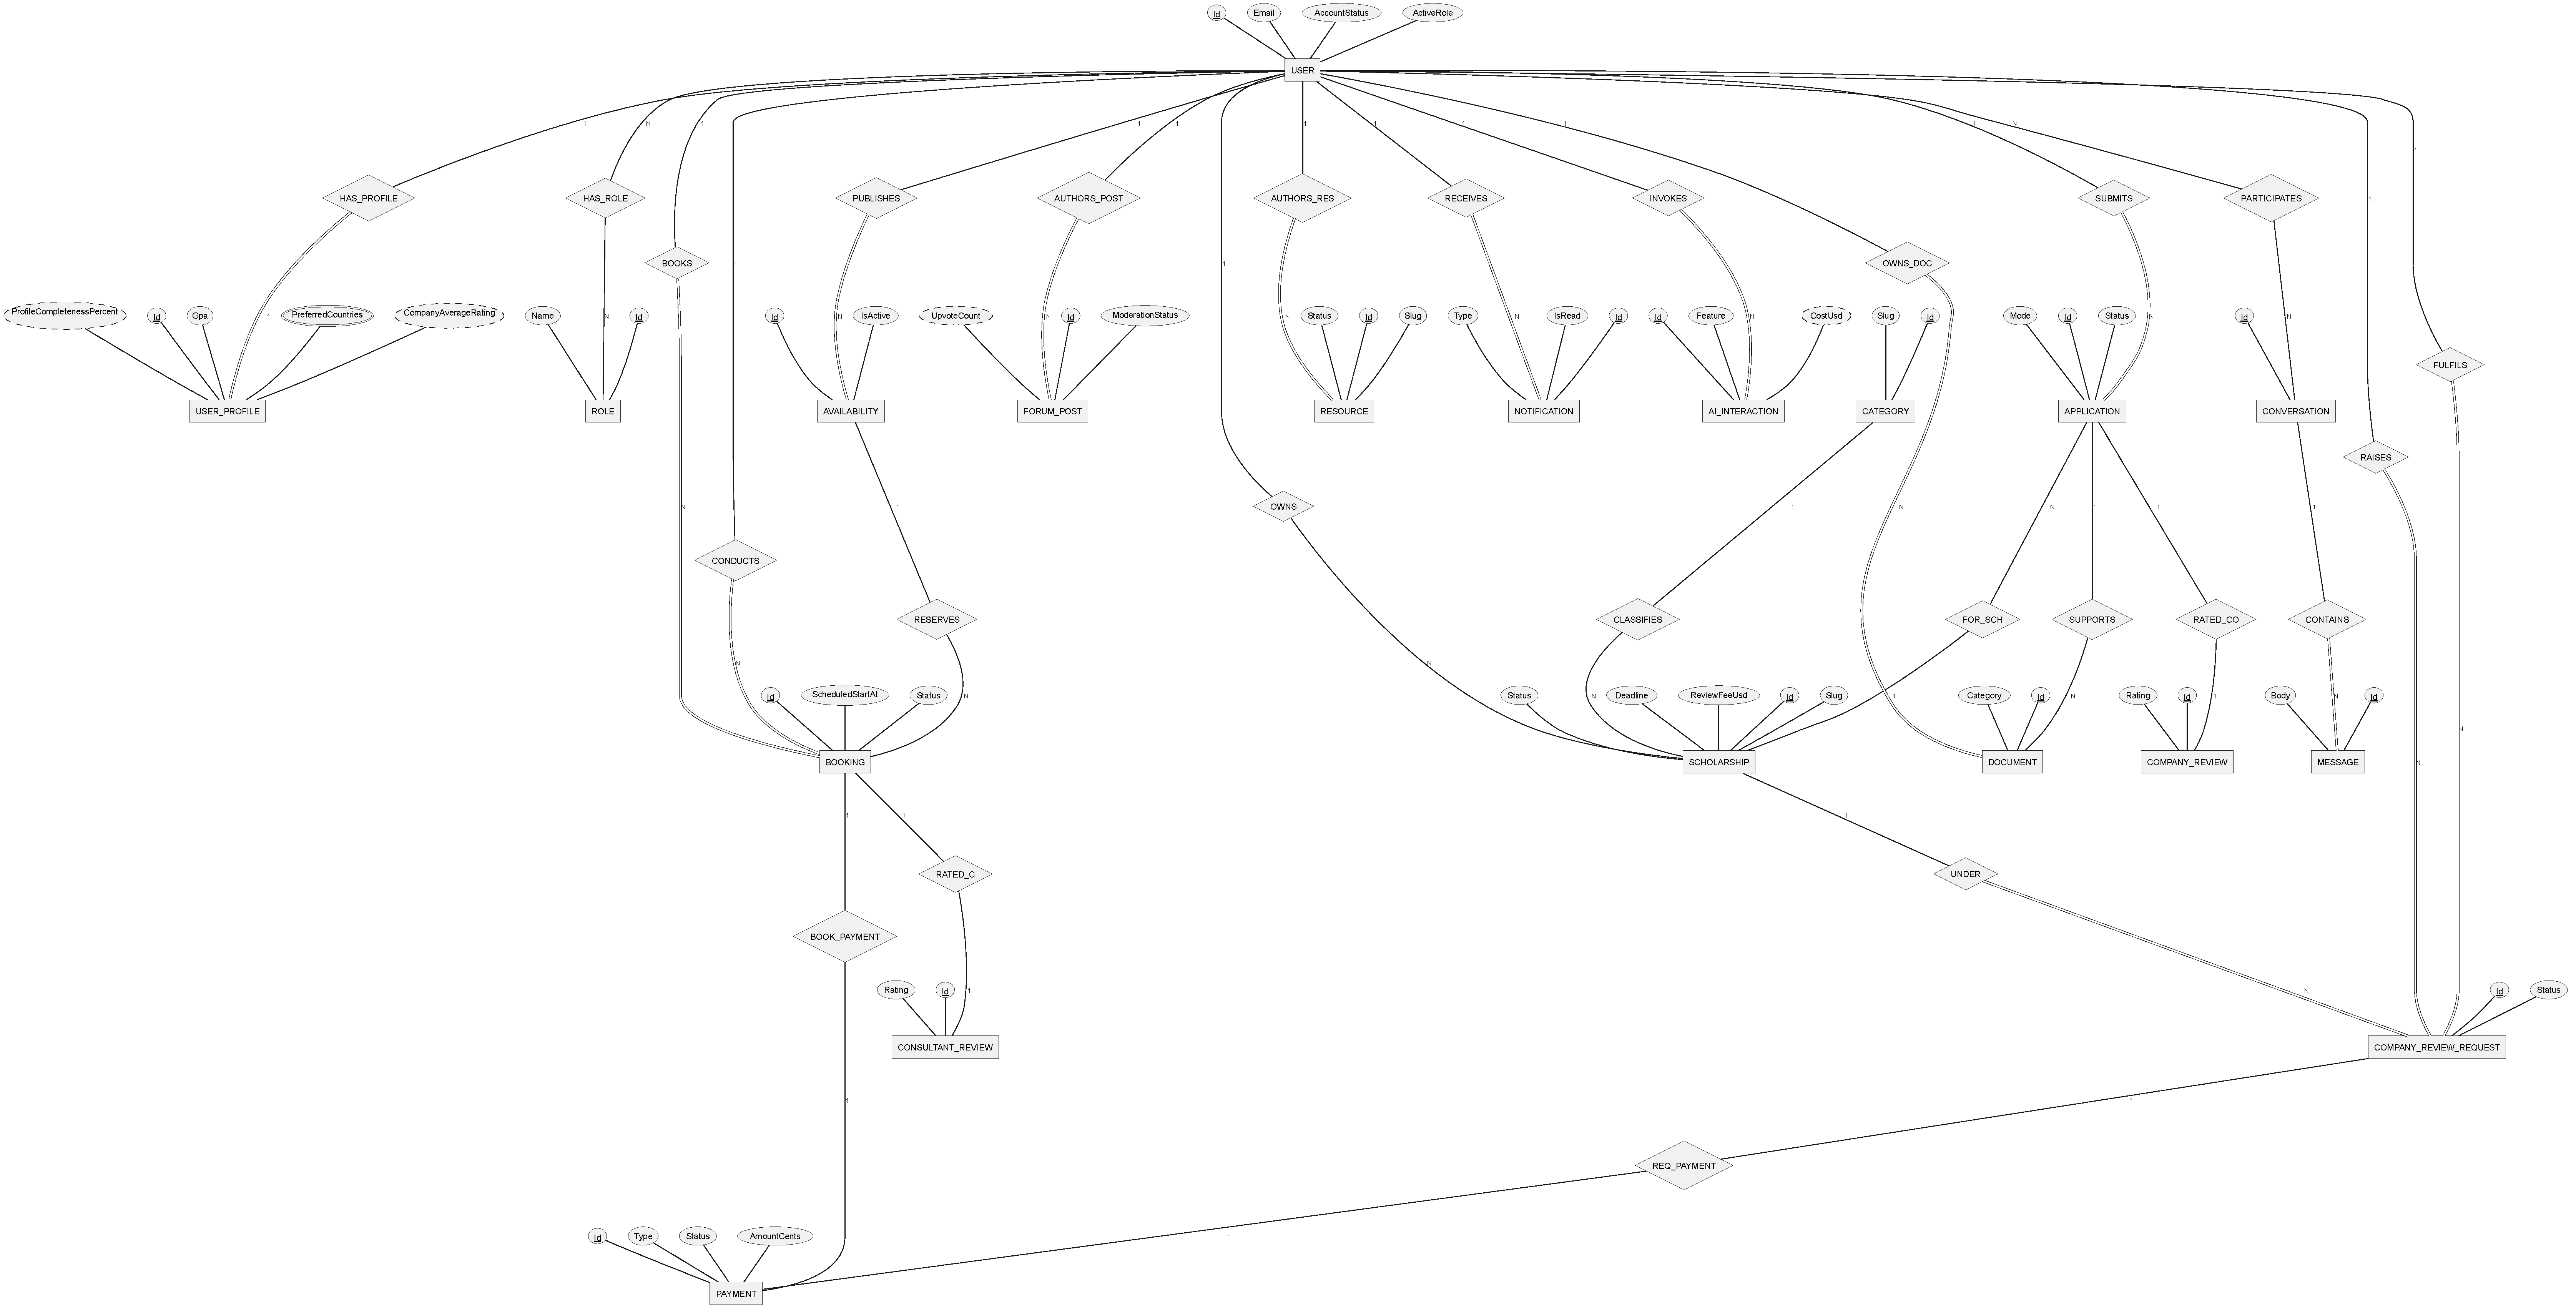
\includegraphics[width=\linewidth,height=0.82\textheight,keepaspectratio]{ScholarPath_EERD_Core.pdf}
\caption{ScholarPath conceptual EERD in Chen / Elmasri notation. Everything
radiates from \texttt{USER}; note the multivalued \texttt{PreferredCountries} and
the derived \texttt{CompanyAverageRating}, \texttt{UpvoteCount},
\texttt{ProfileCompletenessPercent} and \texttt{CostUsd}.}
\label{fig:core}
\end{figure}

\subsection{Identity, Access and Profile}
\label{sec:cluster-identity}

This cluster holds the \texttt{USER} superclass, the \texttt{ROLES} /
\texttt{USER\_ROLES} membership that realises the overlapping specialization, the
1:1 \texttt{USER\_PROFILE} (carrying every role's attributes as nullable
columns), the weak \texttt{EDUCATION\_ENTRIES}, the auth tokens
(\texttt{REFRESH\_TOKENS}, \texttt{PASSWORD\_RESET\_TOKENS}) and the
\texttt{UPGRADE\_REQUESTS} flow with its weak file / link children. The
standalone \texttt{EXPERTISE\_TAGS} taxonomy is referenced only through a
denormalized JSON column, so it carries no relationship edge.

\begin{figure}[H]\centering
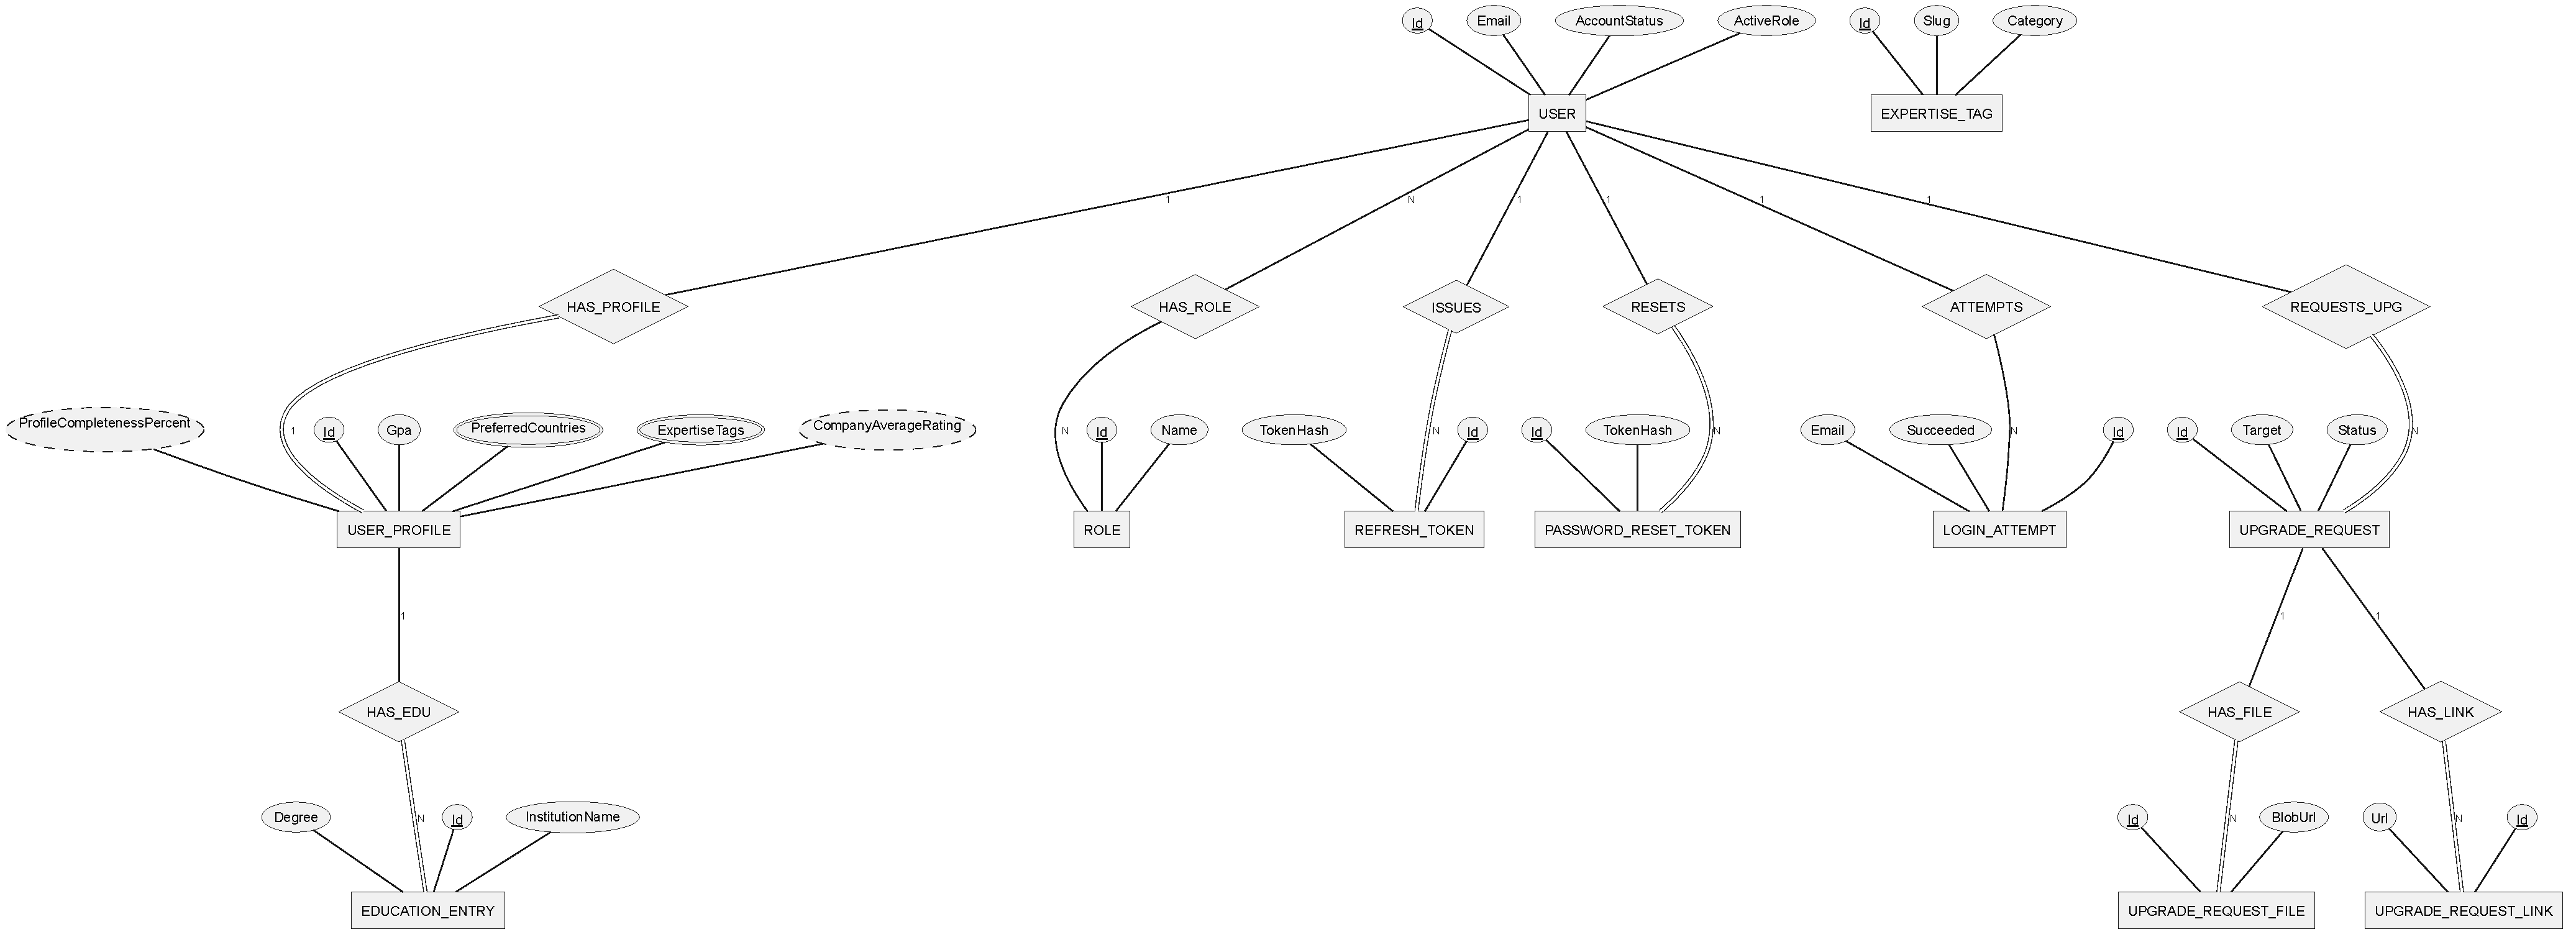
\includegraphics[width=\linewidth,height=0.82\textheight,keepaspectratio]{EERD_Identity_Profile.pdf}
\caption{Identity, Access \& Profile cluster (Chen / Elmasri notation).}
\label{fig:identity}
\end{figure}

\subsection{Scholarships, Applications and Documents}

The academic core: \texttt{CATEGORIES} classify \texttt{SCHOLARSHIPS} (owned
optionally by a Company), students \texttt{SUBMIT} \texttt{APPLICATIONS}, and
\texttt{DOCUMENTS} support applications. Paid expert feedback is modelled by
\texttt{COMPANY\_REVIEW\_REQUESTS} (settled by a \texttt{PAYMENT}) and the 1:1
\texttt{COMPANY\_REVIEWS}. Note the weak \texttt{SCHOLARSHIP\_CHILDREN} and
\texttt{APPLICATION\_CHILDREN} (cascade), and that the single-active-application
rule is enforced in application code rather than by a DB index.

\begin{figure}[H]\centering
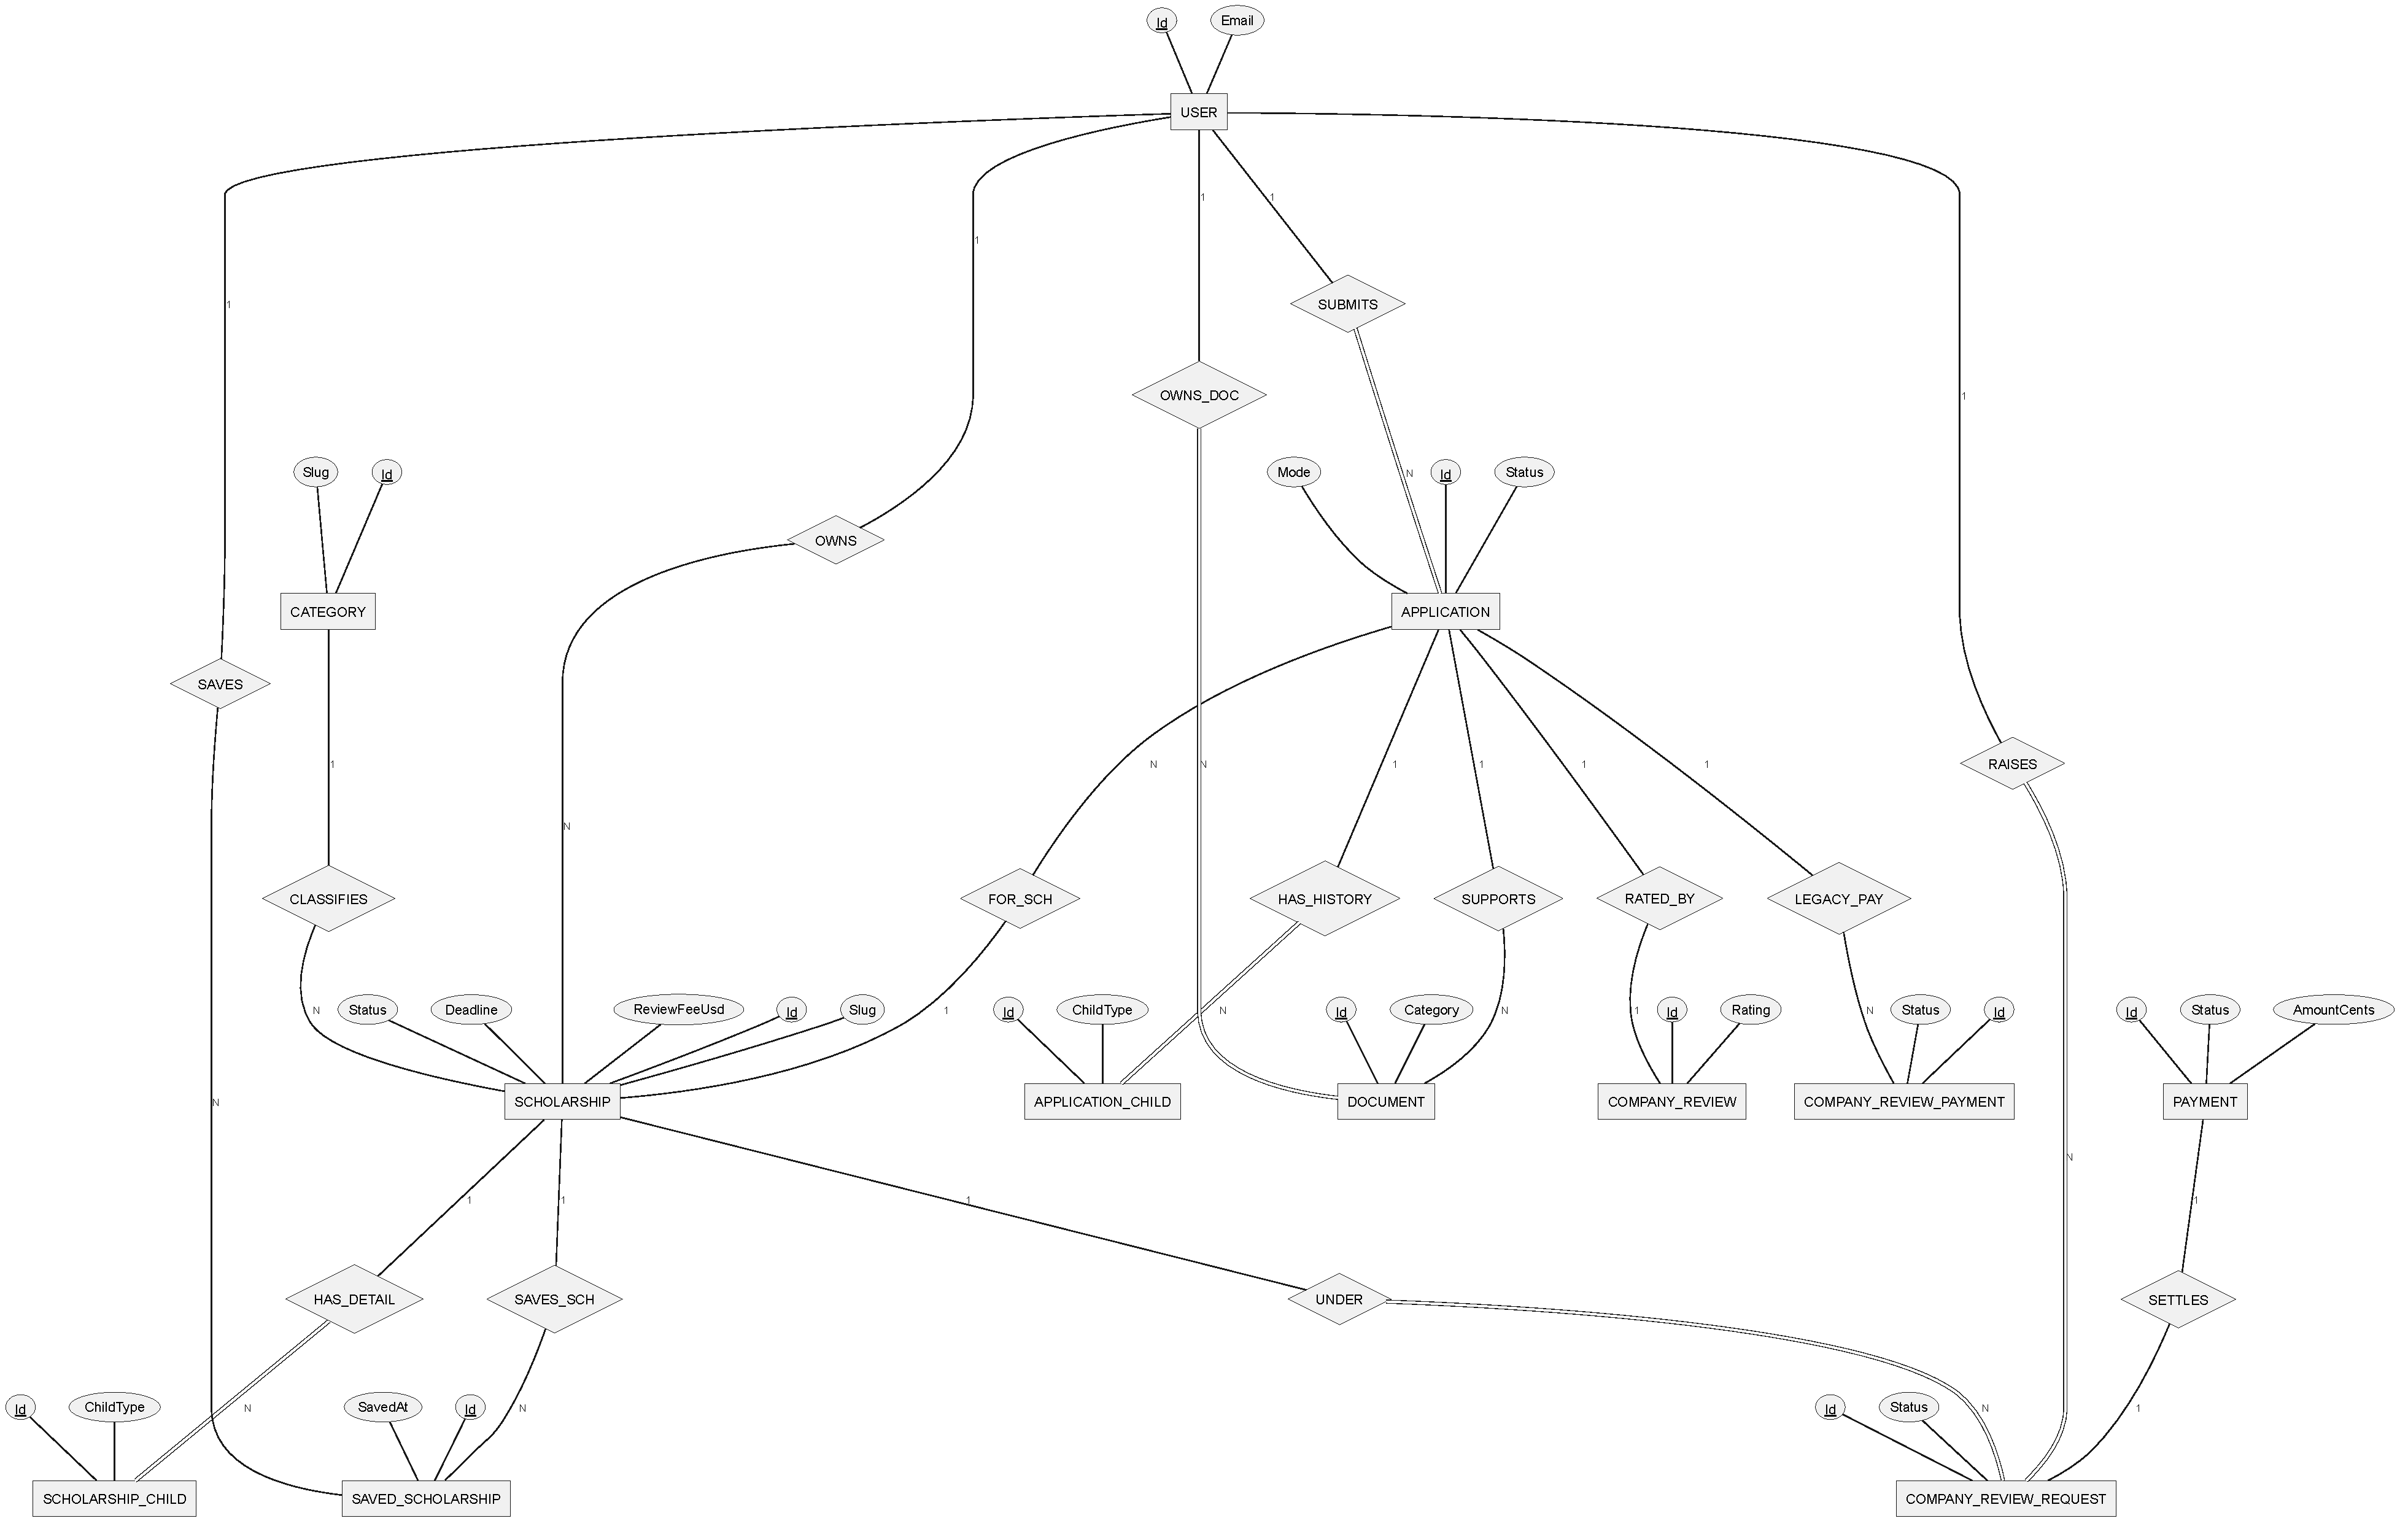
\includegraphics[width=\linewidth,height=0.82\textheight,keepaspectratio]{EERD_Scholarships_Applications.pdf}
\caption{Scholarships, Applications \& Documents cluster (Chen / Elmasri
notation).}
\label{fig:scholarships}
\end{figure}

\subsection{Booking, Payments and Ratings}

Consultants \texttt{PUBLISH} \texttt{AVAILABILITIES}; students \texttt{BOOK}
sessions that consultants \texttt{CONDUCT}; each \texttt{BOOKING} is optionally
settled by a \texttt{PAYMENT}, rated by a 1:1 \texttt{CONSULTANT\_REVIEW}, and
recorded as \texttt{SESSION\_RECORDINGS}. Critically, \texttt{PAYMENT} and
\texttt{PAYOUT} attach to payer, payee, booking and application via
\emph{loose} (dashed) references only --- by design, so settlement history
survives user deletion.

\begin{figure}[H]\centering
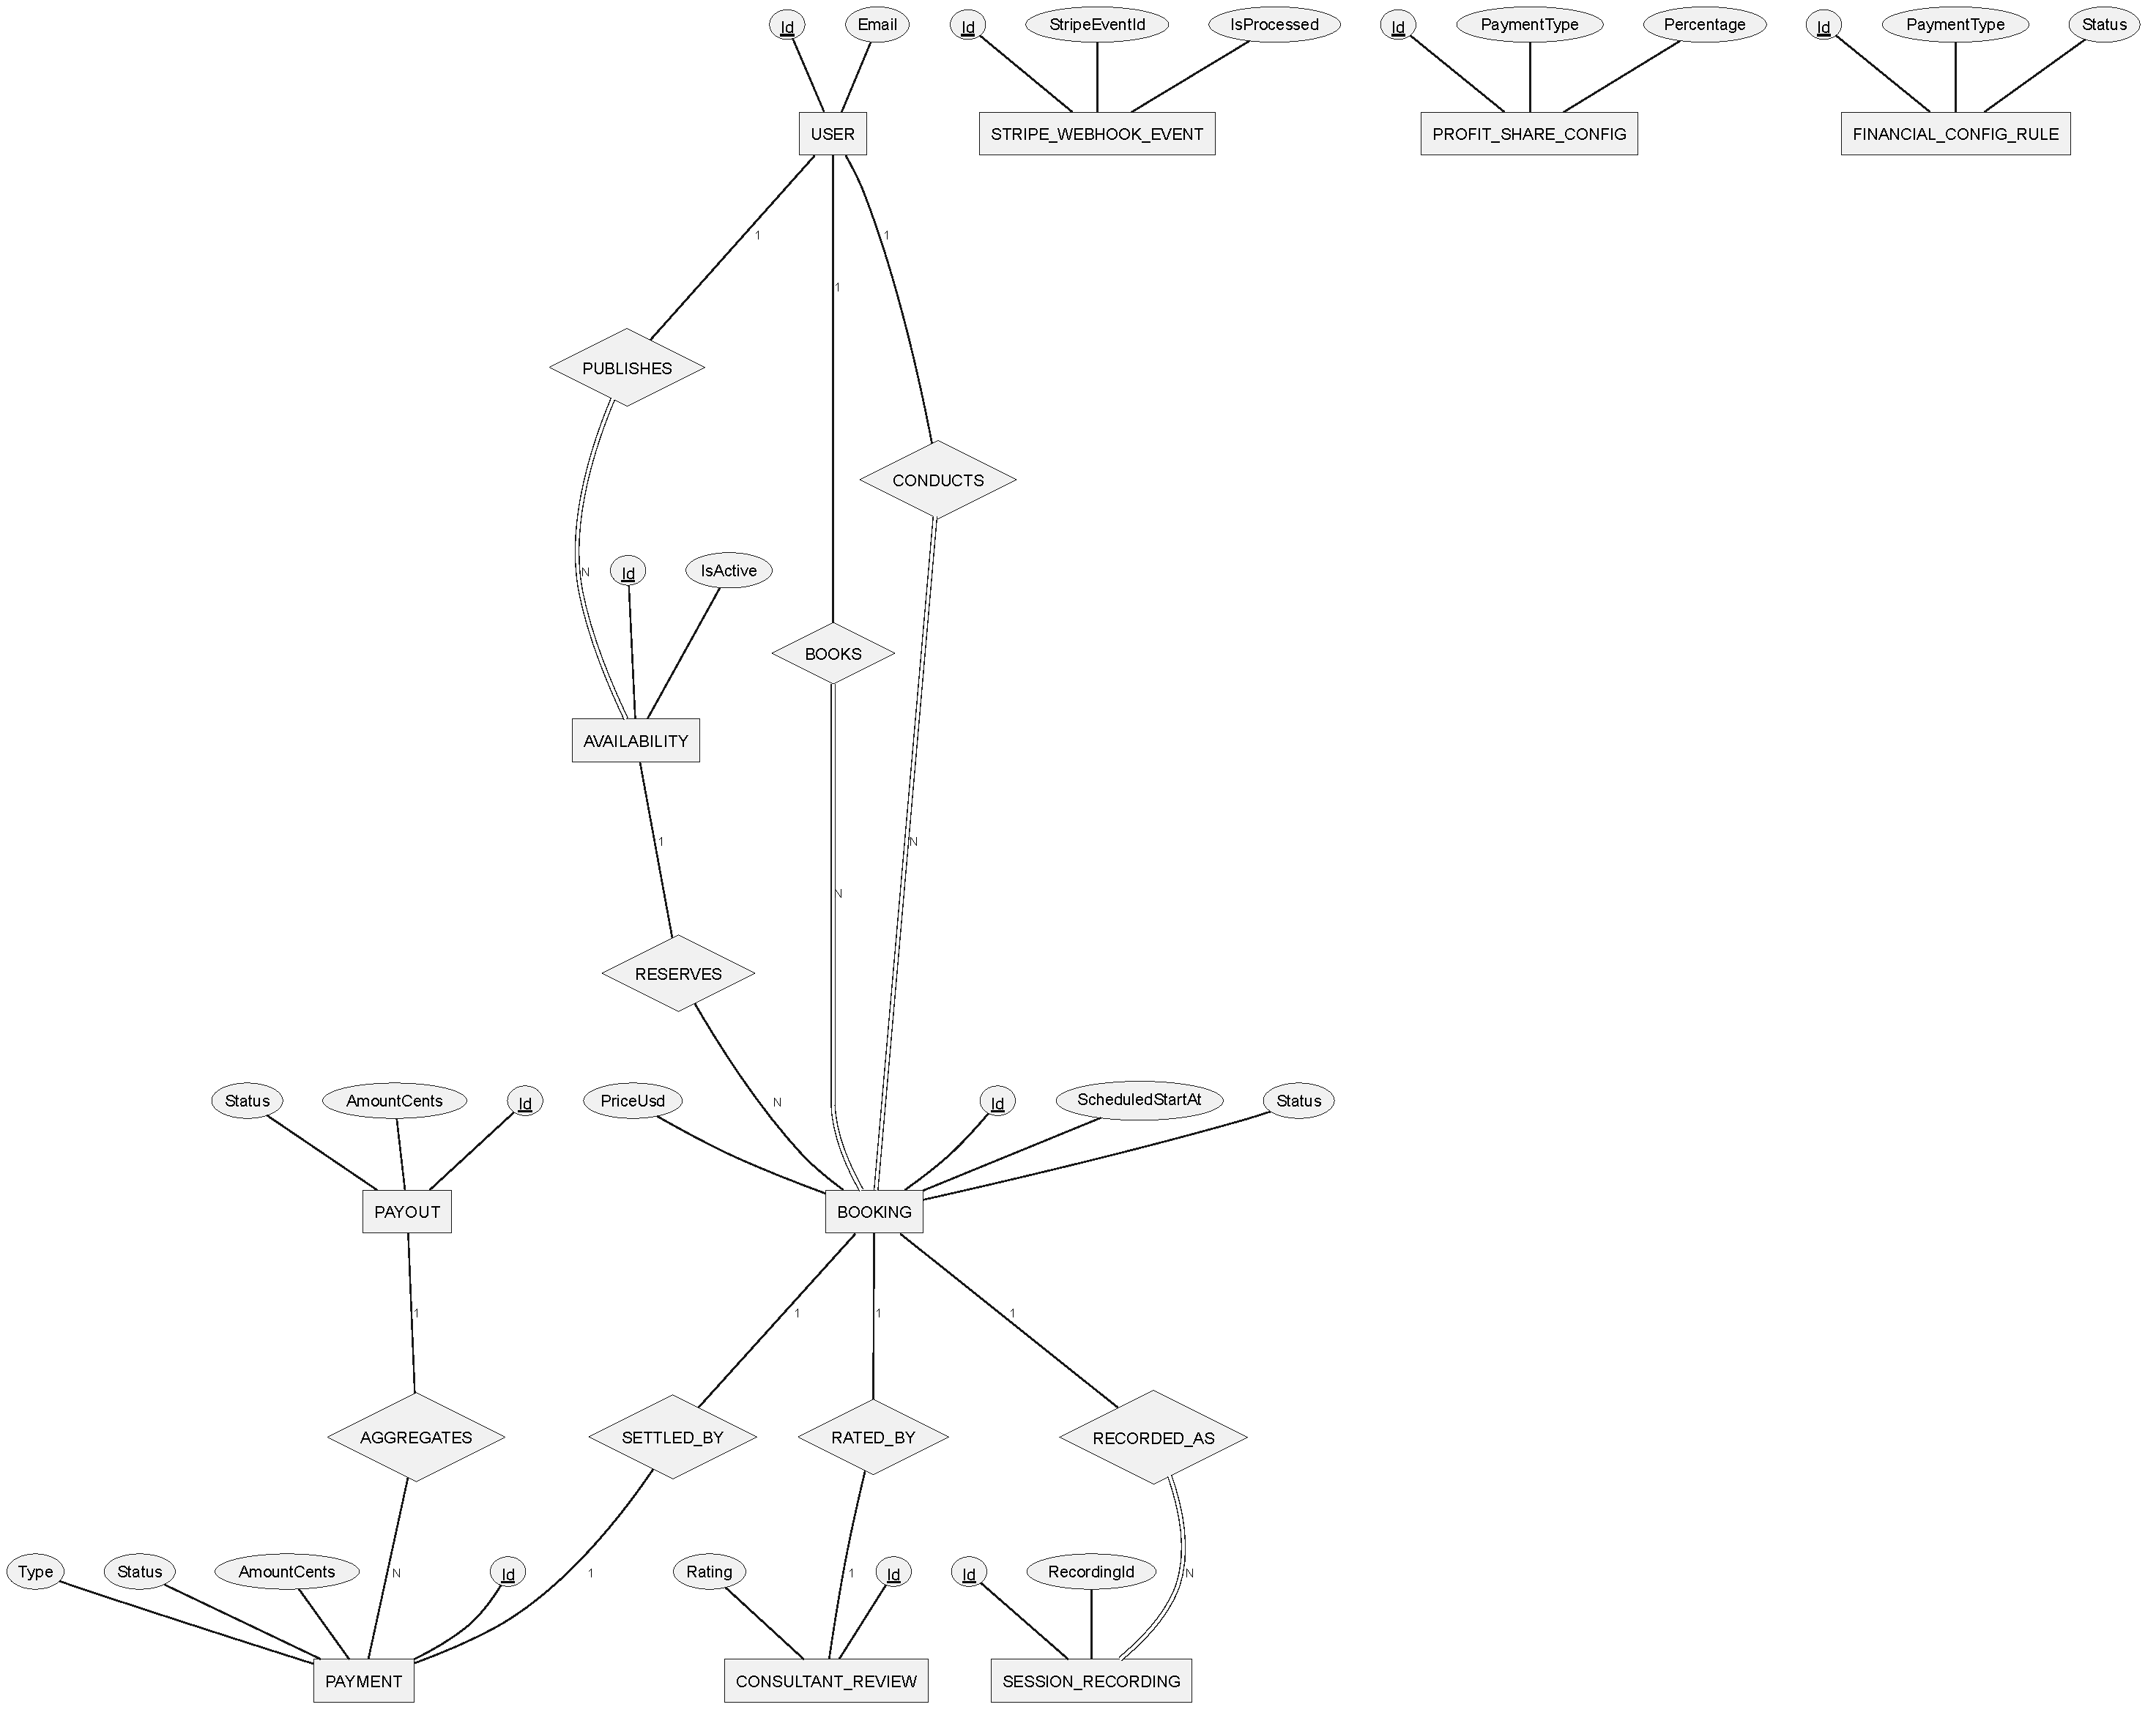
\includegraphics[width=\linewidth,height=0.82\textheight,keepaspectratio]{EERD_Booking_Payments_Ratings.pdf}
\caption{Booking, Payments \& Ratings cluster (Chen / Elmasri notation).}
\label{fig:booking}
\end{figure}

\subsection{Community and Chat}

\texttt{FORUM\_POSTS} (self-referencing for replies) are grouped by
\texttt{FORUM\_CATEGORIES}, tagged through the pure M:N junction
\texttt{FORUM\_POST\_TAGS}, and receive votes, flags and bookmarks --- each
carrying a composite unique key ``one per user per post''. Private messaging is
modelled by \texttt{CONVERSATIONS} (a unique participant pair) containing
\texttt{MESSAGES}. Votes, chat and blocks use loose user references.

\begin{figure}[H]\centering
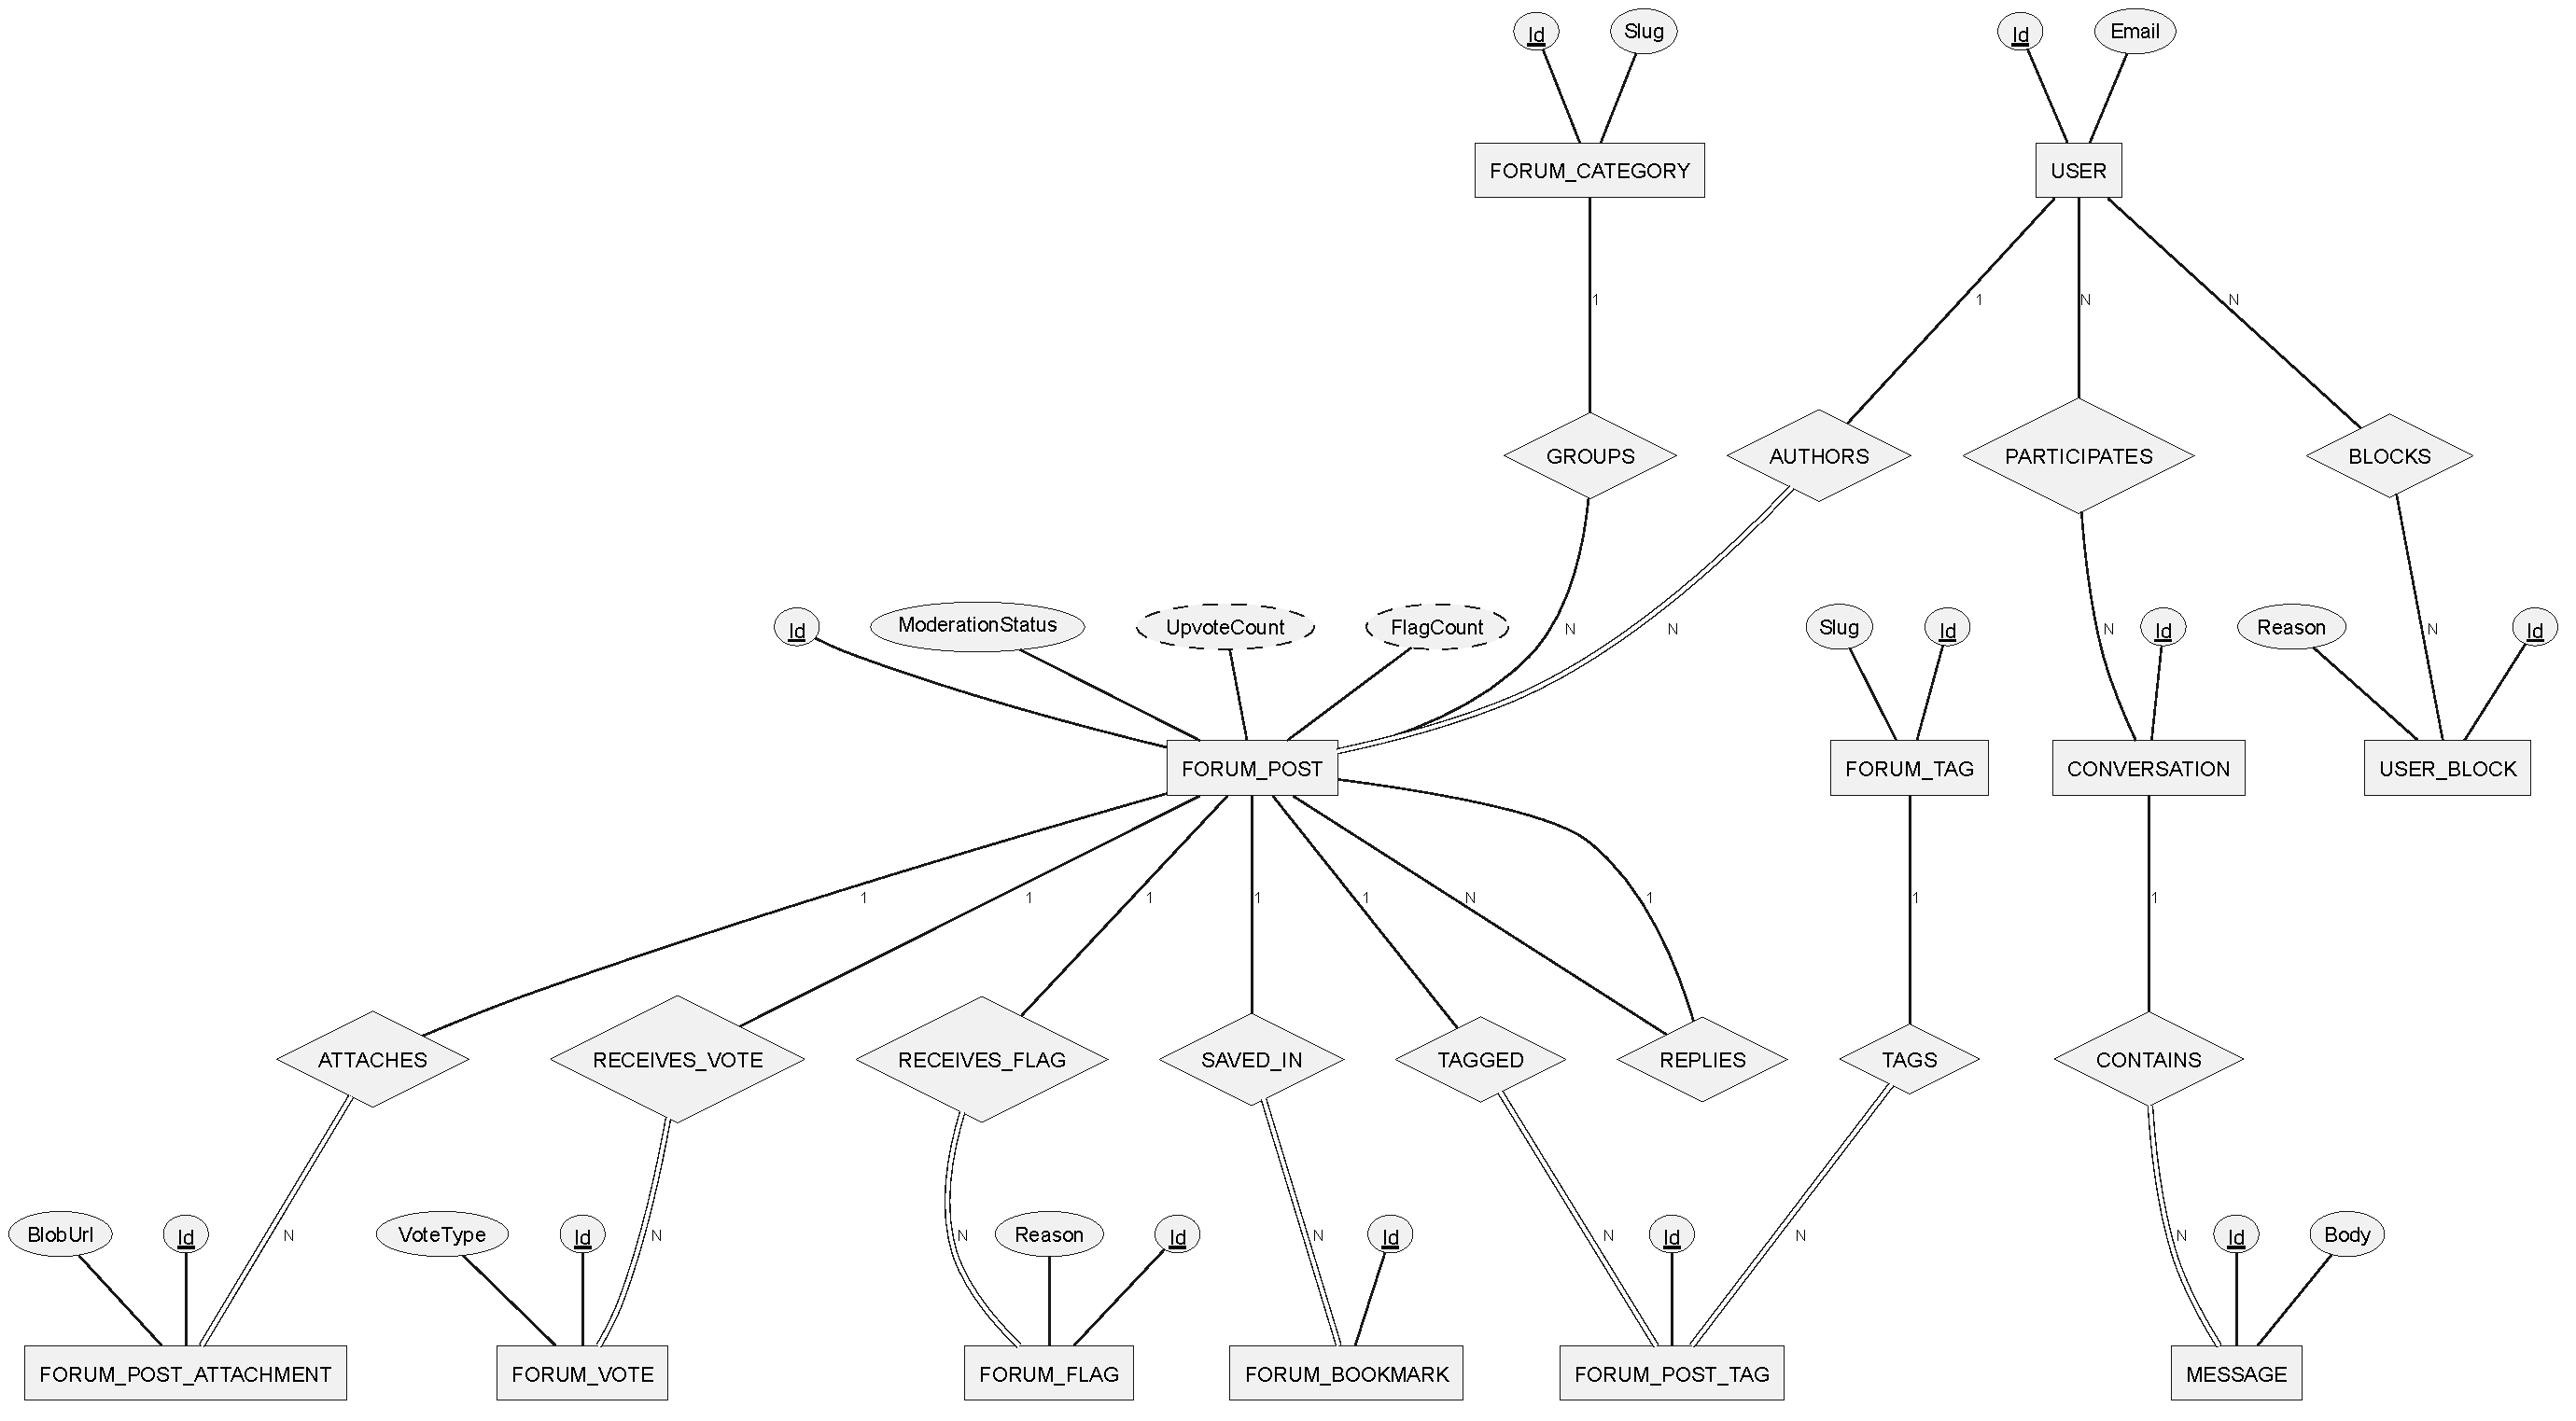
\includegraphics[width=\linewidth,height=0.82\textheight,keepaspectratio]{EERD_Community_Chat.pdf}
\caption{Community \& Chat cluster (Chen / Elmasri notation).}
\label{fig:community}
\end{figure}

\subsection{Resources and Notifications}

The Resources Hub: \texttt{RESOURCES} split into weak
\texttt{RESOURCE\_CHAPTERS}, with per-user \texttt{RESOURCE\_BOOKMARKS} and
\texttt{RESOURCE\_PROGRESS} (and its per-chapter progress children). Delivery is
handled by \texttt{NOTIFICATIONS} and per-type/-channel
\texttt{NOTIFICATION\_PREFERENCES}; both attach to the recipient via loose
references, consistent with the high-volume convention of
Section~\ref{sec:notation}.

\begin{figure}[H]\centering
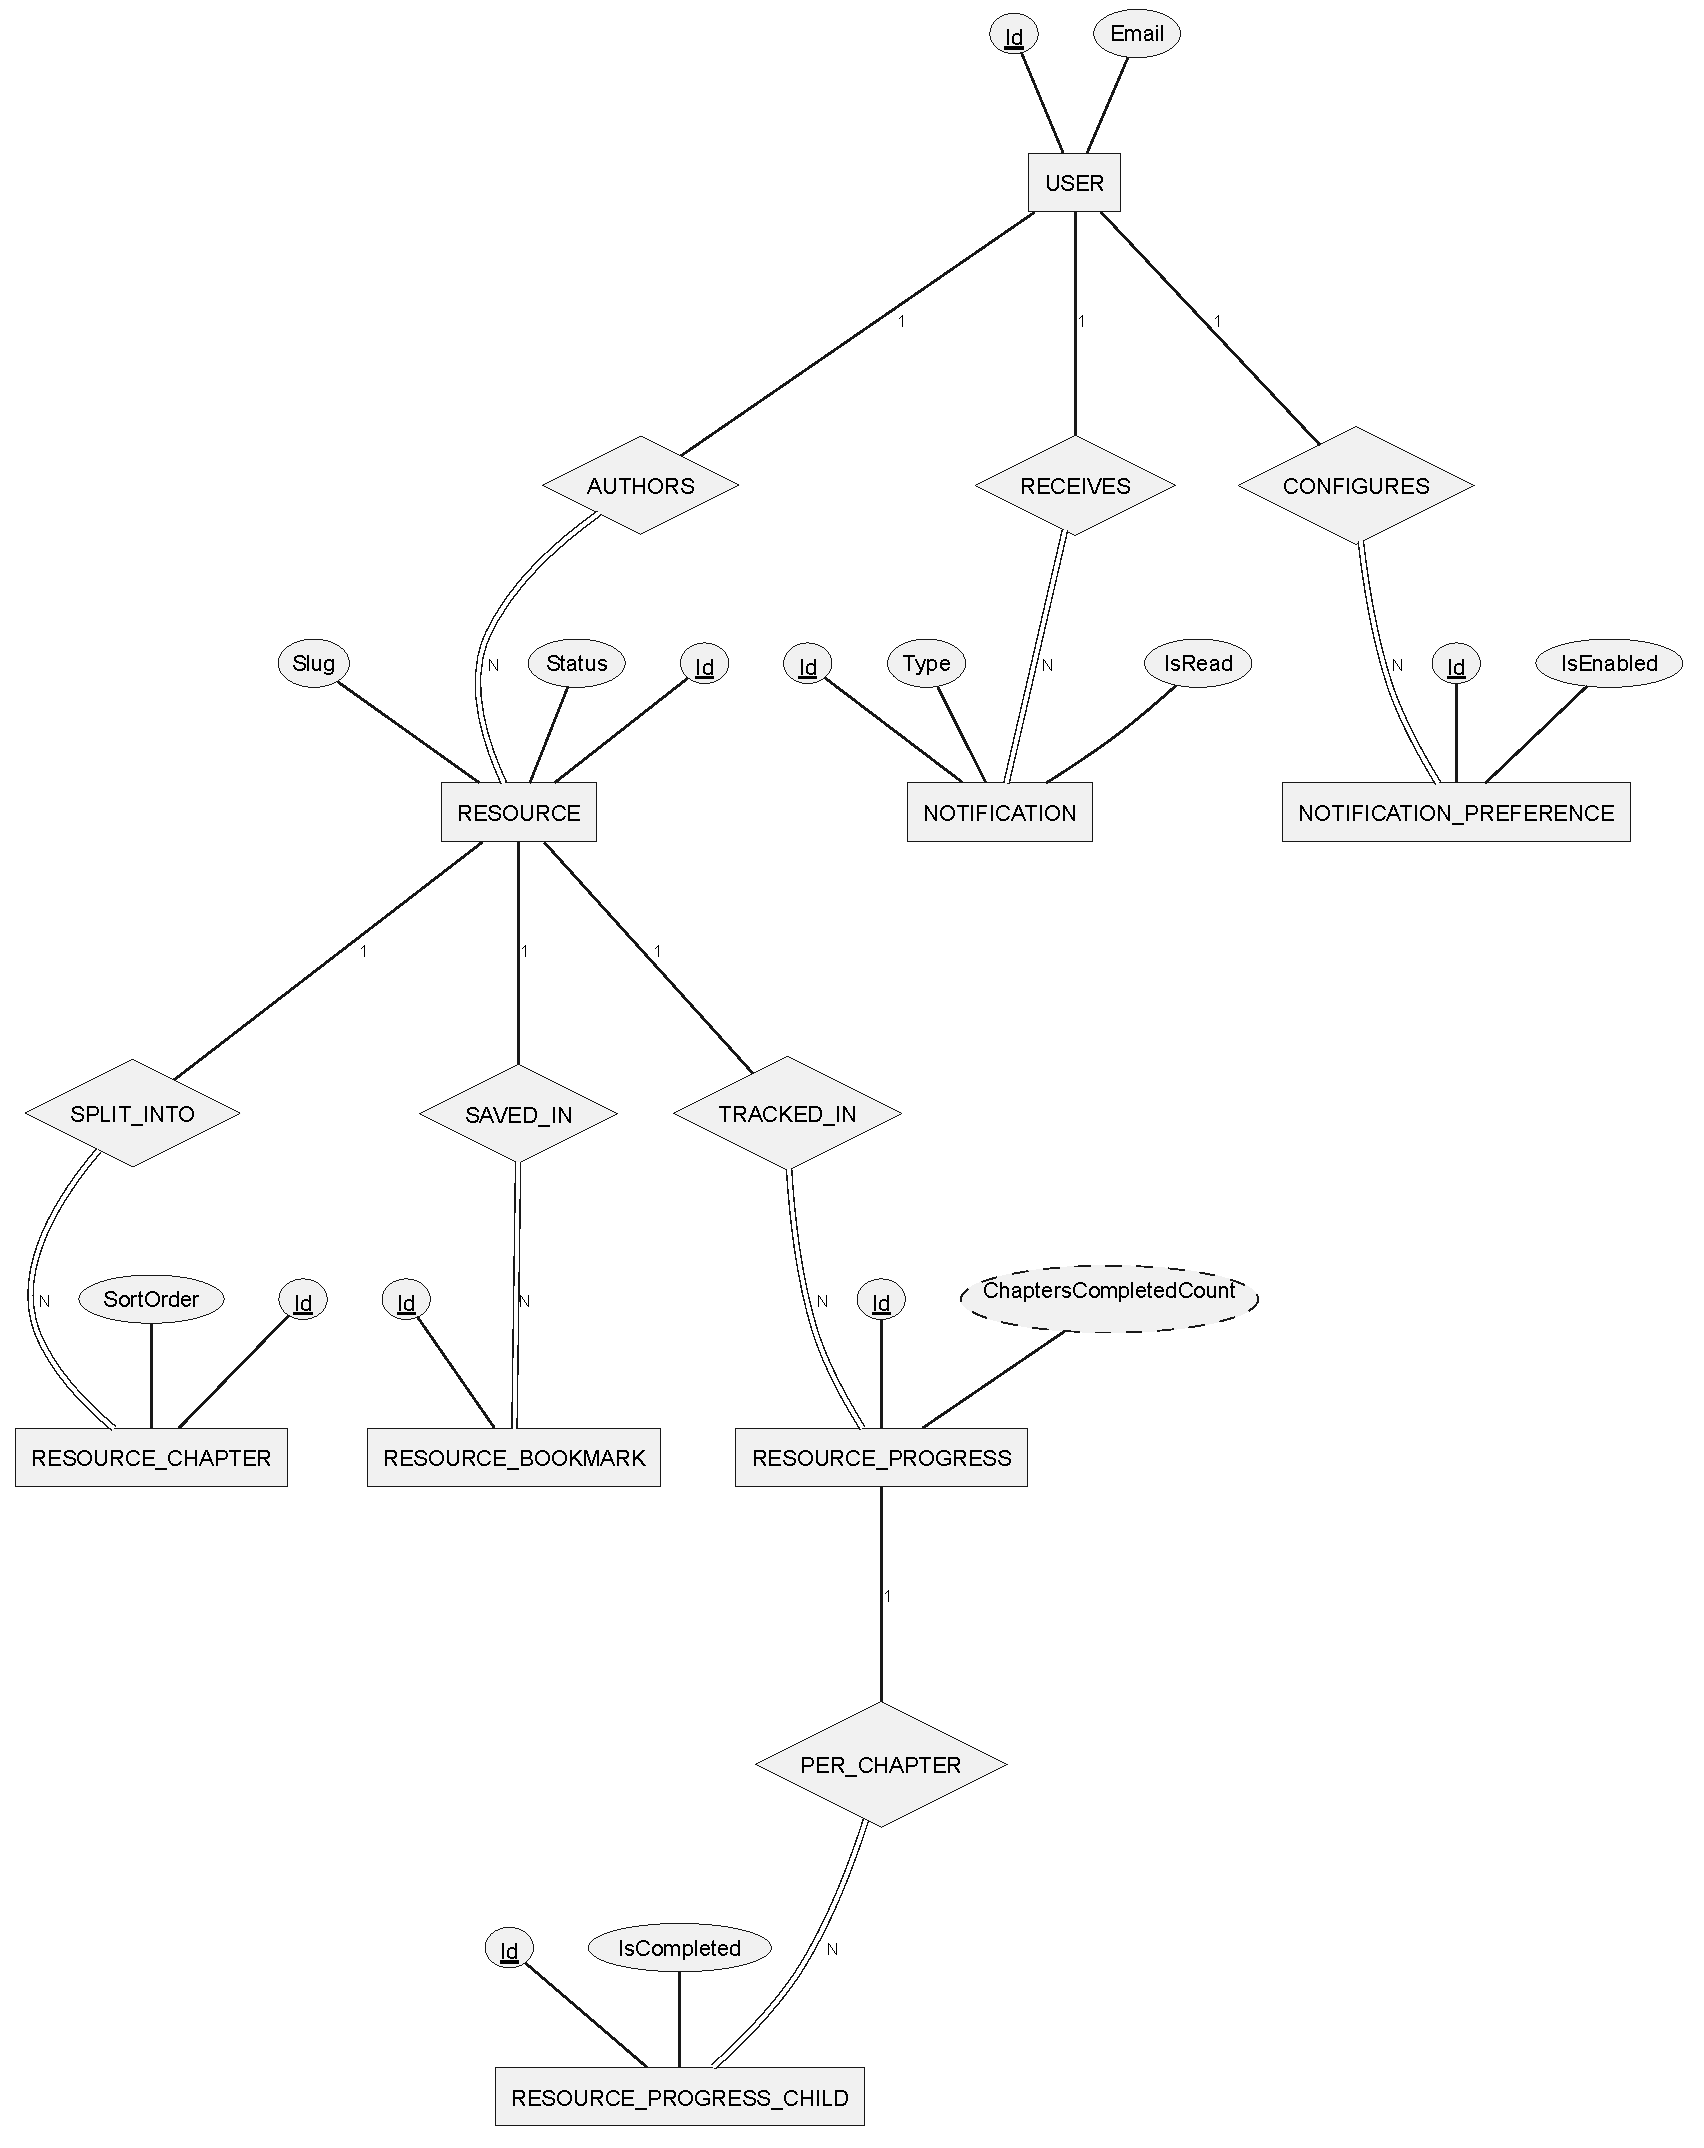
\includegraphics[width=\linewidth,height=0.82\textheight,keepaspectratio]{EERD_Resources_Notifications.pdf}
\caption{Resources Hub \& Notifications cluster (Chen / Elmasri notation).}
\label{fig:resources}
\end{figure}

\subsection{AI, Knowledge Base and Platform}
\label{sec:cluster-ai}

The cross-cutting cluster: \texttt{AI\_INTERACTIONS} (with the derived
\texttt{CostUsd}) feed \texttt{RECOMMENDATION\_CLICK\_EVENTS} and are sampled by
\texttt{AI\_REDACTION\_AUDIT\_SAMPLES}; \texttt{USER\_RISK\_FLAGS} score users
1:1. \texttt{KNOWLEDGE\_DOCUMENTS.SourceId} and \texttt{AUDIT\_LOGS.(TargetType,
TargetId)} are \emph{polymorphic} references --- the category / union construct of
Section~\ref{sec:apply} --- realised as loose id columns because they can point at
any entity type and so cannot be a single FK.

\begin{figure}[H]\centering
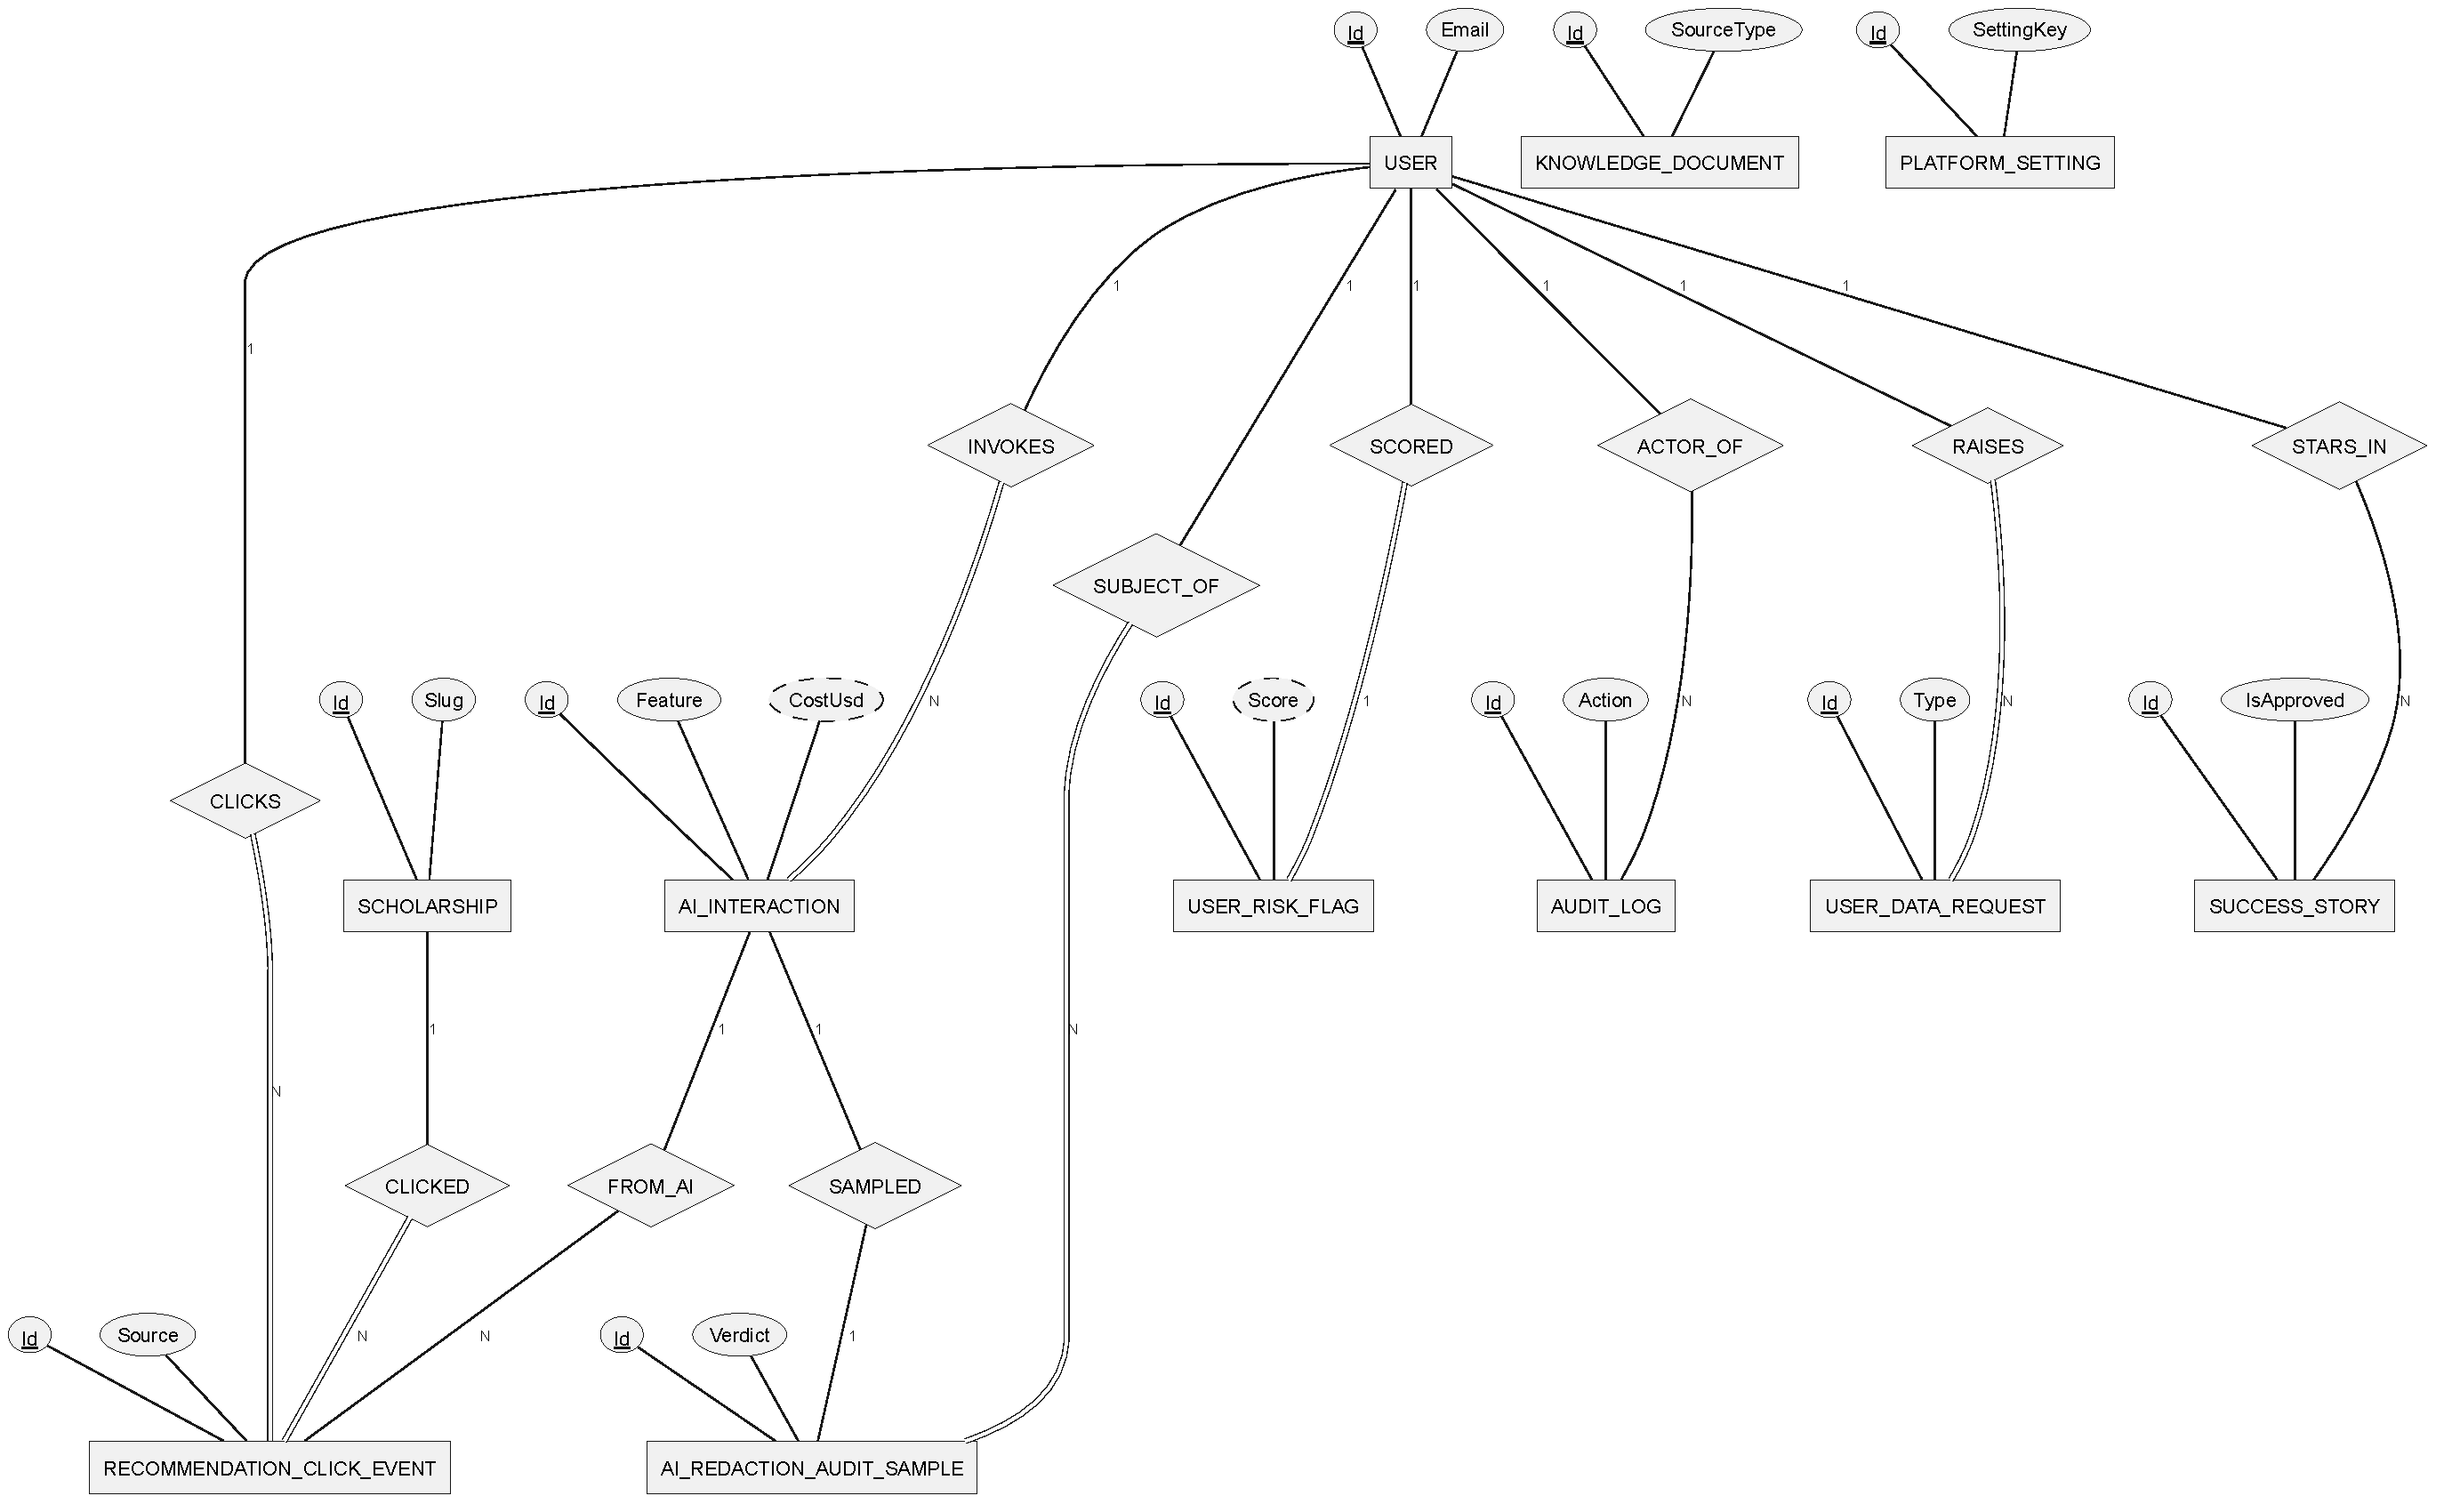
\includegraphics[width=\linewidth,height=0.82\textheight,keepaspectratio]{EERD_AI_Knowledge_Platform.pdf}
\caption{AI, Knowledge Base \& Platform cluster (Chen / Elmasri notation).}
\label{fig:ai}
\end{figure}

\section{Conclusion and Next Step}

We have taken the plain ERD of Part~1 and enriched it into a full EERD. The
headline enhancement is the \texttt{USER} specialization --- \emph{overlapping}
(dual roles) and \emph{partial} (an Unassigned newcomer belongs to no subclass)
--- physically realised as a single \texttt{Users} table plus a
\texttt{UserRoles} join and nullable role columns on \texttt{UserProfiles}. We
also added weak entities (education and child rows, upgrade attachments),
multivalued attributes (preferred countries as JSON), derived attributes
(\texttt{CompanyAverageRating}, \texttt{UpvoteCount},
\texttt{ProfileCompletenessPercent}, \texttt{CostUsd}), categories (the two
polymorphic references), and the project-specific solid-versus-dashed edge
convention.

\textbf{Next: Part~3 --- Relational Mapping.} Having a faithful conceptual EERD,
we now translate it into actual relations: turning entities into tables, choosing
primary and foreign keys, mapping the single-table specialization, breaking out
(or JSON-encoding) multivalued attributes, materialising weak entities as cascade
child tables, and turning each relationship's cardinality and participation into
concrete key placement and delete rules. That table-by-table schema is the
subject of \texttt{02-RELATIONAL-MAPPING.md}.

\end{document}
